\chapter{装饰}

\begin{quote}
    我说,我要上这棕树,抓住枝子。愿你的两乳好像葡萄累累下垂,你鼻子的气味香如苹果。你的口如上好的酒,女子说,为我的良人下咽舒畅,流入睡觉人的嘴中。

    \hfill《圣经·雅歌》7:10
\end{quote}

那本章的主要思路是介绍,介绍那些为生成文档中个别部分而被个性化修改的\LaTeX 的标准工具,间或可以从中看到些用于“调香”的宏。这些个性化设置可以应用于各个层级:使用包的选项,如设置页眉;偶尔涉足宏定义,如设置章节的展现风格;更深入地处理宏,如处理内容的表格。本章的一部分聚焦于我们可以从包\textsf{fancyvrb}中调用的工具。作为本章的末尾,我们会去抨击一下法文的引号。

\section{索引的外观} % 这节翻译得是什么破玩意

为了修改索引的外观,需要明白,当我们大手一挥噼里啪啦地写下如下指令的时候,我们实际上就生成了一个文件\codereplace{文档}\dm{.ind}:

\dmh{makeindex }\codereplace{文档}

该文件包含了类似下面列出的内容:

\begin{dmd}
\verb|\begin{theindex}| \quad$\leftarrow$\textsf{文前部分}\\
~\\
\verb|\item Cosmic debris, 12,34|\\
~\\
\verb|\indexspace| \quad$\leftarrow$\textsf{分组间的空间}\\
~\\
\verb|\item Debra kadabra, 23| \quad$\leftarrow$\textsf{入口,分割符,页码}\\
~\\
\verb|\end{theindex}| \quad$\leftarrow$\textsf{文后部分}
\end{dmd}

实际上,该代码会从带有预定义值且可被修改的一般性实体中生成。为了证明这个观点,只需要知道,程序\textsf{makeindex}可以生成一个包含\LaTeX 代码外内容的\dm{.ind}文件。为了理解一般性实体的职责,可以用如下方式描述\textsf{makeindex}的工作。

\begin{enumerate}
    \item 根据实体\dm{preamble}的值来写入文前部分。
    \item 对于每个\dm{.idm}文件:
    \begin{enumerate}
        \item 写入实体\dm{item\_0}的内容;
        \item 写入入口(本例中为“Cosmic debris”);
        \item 写入分割符(实体\dm{delin\_0}的值);
        \item 写入页码。
    \end{enumerate}
    \item 在每个分组的结尾(即首字母切换时),写入实体\dm{group\_skip}的内容;
    \item 根据\dm{postamble}的值写入文后部分。
\end{enumerate}

上述实体的默认值如下:

\begin{center}
    \begin{dmd}
        \begin{tabular}{|l|l|}
            \hline
            preamble & \verb+"\\begin{theindex}\n"+\\
            item\_0 &\verb+"\n \\item"+\\
            delim\_0 & ", "\\
            group\_skip & \verb+"\n\n \\indexspace\n"+\\
            postamble & \verb+"\n\n\\end{theindex}\n"+\\
            \hline
        \end{tabular}
    \end{dmd}
\end{center}

这些值可以使用通常带有后缀名\dm{.ist}的风格文件作为媒介来修改。可以通过以下方式在调用\textsf{makeindex}时使用:

\dmh{makeindex -s \codereplace{风格}.ist \codereplace{文件}}

如此一来,为了生成文档的标题,我们可以一开始就重新定义一二级间的分隔符:

\begin{dmd}
\begin{verbatim}
delim_0 " \\dotfill \ "
delim_1 " \\dotfill \ "
\end{verbatim}
\end{dmd}

我们将默认用于分隔索引入口和页码的逗号替换成了省略号。接下来,通过严谨地阅读\textsf{makeindex}的文档\jz{
    可参见参考文献的实用引用后的提醒。
},可以注意到要求\textsf{makeindex}为入口组和代表分组的字母间生成空间的礼貌方式如下:

\begin{dmd}
headings\_flag 1
\end{dmd}

这里,代表分组的字母会表示为大写,并且借助实体\dm{heading\_prefix}和\dm{heading\_suffix}的内容框起。无所谓——为了生成我们美丽的带阴影的字盒,我们可以在风格文件中这样写:

\begin{dmd}
\begin{verbatim}
heading_prefix "{\\large\\sffamily\\bfseries\\shadowbox{"
heading_suffix "}\\hfill}\\nopagebreak\n"
\end{verbatim}
\end{dmd}

这段你已经可以看懂的示例内容,就会生成我们需要的字盒。例如对于字母C:

\begin{codelist}[10.1]{
    {\large\sffamily\bfseries%
    \shadowbox{C}\hfil}\nopagebreak
}\begin{verbatim}
{\large\sffamily\bfseries%
    \shadowbox{C}\hfil}\nopagebreak
\end{verbatim}
\end{codelist}

这段指令会被\dm{group\_skip}的内容覆盖掉。而我们稍早前说过,\dm{group\_skip}的默认值是\verb|\indexspace|。在研究了几个月之后\jz{
    开玩笑的。我是想说,只花了几秒……好吧,几分钟。
},我们成功地在\dm{book.cls}中发现了该指令的定义,并且将分组间空间略微扩大了些:

\begin{dmd}
\renewcommand\indexspace{%
    \par \vskip 20pt plus5pt minus3pt\relax}
\end{dmd}

\begin{ii}
本小节中,我们只是非常简单地看了看makeindex提供的功能。除了在《\LaTeX 伴侣》中能找到的信息,Debian环境下关于此工具的说明书中提供了我们可以定义的一半入口的详尽列表。由P.陈(P. Chen;音译)和M.A.哈林森(M. A. Harrinson)编写的文件\dm{ind.dvi}同样是初学索引自定义的良好开端。
\end{ii}

\section{标题的外观}

在本节,我们会介绍我们修改\LaTeX 标准(篇、章、节等)标题外观的方式。

\subsection{目录中的编号}

作为开始操作目录的前提条件,需要掌握两个计数器:

\begin{enumerate}
    \item \dm{secnumdepth}(英:\emph{section numbering depth}),可以明确文档中标题编号的层级;
    \item \dm{tocdepth}(英:\emph{table of contents depth}),可以定义目录标题的最大层级(或称最大深度)。
\end{enumerate}

为了使用这两个计数器,还需要了解\LaTeX 为各标题连接层级的方法。以下是各标题的层级:

\begin{center}
    \begin{tabular}{|c|r||c|r|}
        \hline
        标题 & 层级 & 标题 & 层级\\
        \hline
        \dm{part} & -1 & & \\
        \dm{chapter}    & 0 & \dm{subsubsection} & 3\\
        \dm{section}    & 1 & \dm{paragraph}     & 4\\
        \dm{subsection} & 2 & \dm{subparagraph}  & 5\\
        \hline
    \end{tabular}
\end{center}

如此一来,将\verb|secnumdepth|赋值为1、将\verb|tocdepth|赋值为2,则可以让标题编号至各\verb|\section|,同时将层级少于\verb|\subsection|的标题插入目录。

\subsection{节和更少的层级}

在\TeX 系统的文件\dm{book.cls}中,我们可以找到如下代码\jz{
    稍微简化了一些……
}:

\begin{dmd}
\begin{verbatim}
\newcommand{\section}{%
    \@startsection%
    {section} % 标题名称
    {1} % 标题层级
    {0pt} % 缩进
    {-3.5ex plus -1ex minus -.2ex}% 段前纵向空间
    {2.3ex plus.2ex}% 段后纵向空间{\normalfont\Large\bfseries}} % 标题外观
\end{verbatim}
\end{dmd}

该段代码定义了节标题的生成方式。可以观察到,指令\verb|\section|调用了指令\verb|\@startsection|,而后者需要6各参数:

\begin{itemize}
    \item 标题名称,如\dm{section}、\dm{subsection}等;
    \item 标题层级,1对应\dm{section},2对应\dm{subsection},3对应\dm{subsubsection},等等;
    \item 缩进;
    \item 标题前的纵向空白;
    \item 标题后的纵向空白;
    \item 用于确定标题本身格式的一系列\emph{声明}。
\end{itemize}

因此,我们可以注意到\LaTeX 默认为类型\dm{book}设定的版式如下。

\begin{itemize}
    \item 无缩进(\dm{0pt})。
    \item 标题前的纵向空间为\dm{3.5ex},带有正向\dm{-1ex}和负向\dm{-.2ex}的允差。
    \item 标题后的纵向空间为\dm{2.3ex},带有正向\dm{.2ex}的允差。可以注意到,如果空间为负,则段落开头会紧接标题,而不会重起一段。
    \item 标题加粗加大,使用“常规”(normal)字体。
\end{itemize}

为了定义本文档使用的标题样式,我们引入三个长度,分别用于\dm{section}、\dm{subsection}、\dm{subsubsection}的缩进:

\begin{dmd}
\begin{verbatim}
\newlength{\sectiontitleindent}
\newlength{\subsectiontitleindent}
\newlength{\subsubsectiontitleindent}
\end{verbatim}
\end{dmd}

长度值如下:

\begin{dmd}
\begin{verbatim}
\setlength{\sectiontitleindent}{-1cm}
\setlength{\subsectiontitleindent}{-.5cm}
\setlength{\subsubsectiontitleindent}{-.25cm}
\end{verbatim}
\end{dmd}

此外,我们为标题还定义了特殊的字体,具体如下:

\begin{dmd}
\begin{verbatim}
\newcommand{\sectionfont}{% 
    \fontencoding{\encodingdefault}% 
    \fontfamily{pag}% \fontseries{bc}%
    \fontshape{n}% \selectfont}
\end{verbatim}
\end{dmd}

该指令可以选用PostScript字体AvantGarde的加粗紧缩版本(参阅9.4节)%TODO 解释中文的使用
。最终,我们使用了以下指令来定义节标题外观:

\begin{dmd}
\begin{verbatim}
\renewcommand{\section}{% 
    \@startsection%
    {section}%
    {1}%
    {\sectiontitleindent}%
    {-3.5ex plus -1ex minus -.2ex}% 
    {2.3ex plus.2ex}% {\sectionfont\Large}}
\end{verbatim}
\end{dmd}

对于更少层级的标题,我们也编写了等价的指令。

\subsection{章}

通过深入研究文件\dm{book.cls},我们可以找到有关\LaTeX 生成章首内容的信息。

\subsubsection{原则}

在文件\dm{book.cls}中,我们可以找到以下指令:

\begin{dmd}
\begin{verbatim}
\newcommand{\chapter}{% 
    ...
    \thispagestyle{plain}%
    ...
    \secdef\@chapter\@schapter} % 我们感兴趣的行
\end{verbatim}
\end{dmd}

指令\verb|\chapter|本身会调用两个不同的指令:

\begin{enumerate}
    \item \verb|\@chapter|,用于被编号的章标题;
    \item \verb|\@schapter|,用于不被编号的章标题(\dmh{s}代表\emph{star},即“星号”,对应指令\verb|\chapter*|)。
\end{enumerate}

在英勇地(同样在文件\dm{book.cls}中)查找这两条指令的定义之后,我们找到了下面这类东西:

\begin{dmd}
\begin{verbatim}
\def\@chapter[#1]#2{% ...
    \refstepcounter{chapter}%
    % 终端上的消息:
    \typeout{\@chapapp\space\thechapter.} 
    \addcontentsline{toc}{chapter}% 在目录中添加标题
    ...
    \if@twocolumn
    ...
    \else% 针对不分栏的文档
    \@makechapterhead{#2}% 我们感兴趣的代码行
    \fi}
\end{verbatim}
\end{dmd}

这段代码把我们领上道了……实际上,\verb+\@makechapterhead+(可以按字面翻译为“制作章首装饰”)正是我们更改图案所需要重定义的指令。经过进一步的搜索,我们可以发现指令\verb|\@makeschapterhead|能够生成未编号的章首装饰。这两条指令接受章名作为其参数。

\subsubsection{必要的小工具}

我们定义了环境\dm{cadrechap},用于简单地讲右边距加宽2厘米:

\begin{dmd}
\begin{verbatim}
\newenvironment{cadrechap}% 
    {\begin{list}{}{%
        \setlength{\leftmargin}{0pt}% 
        \setlength{\rightmargin}{-2cm}% 宽敞些
        \setlength{\itemindent}{0pt}% 
        \setlength{\labelsep}{0pt}%
    }\item}% 
{\end{list}}
\end{verbatim}
\end{dmd}

同时,可以使用布尔值\dm{@mainmatter}来获取我们目前是否处于文档的“中心”——这是针对指令\verb|\mainmatter|被调用的情况。

\subsubsection{严格的章首装饰}

本文档中,生成章首装饰的指令可以看作两个微型页面的组合。%TODO minipage

\begin{enumerate}
    \item 在左侧的是微型页面字盒。我们指定了它的高度,以便放置微型摘要(参见\S 10.7)。
    \item 在右侧的是包含“章”一词和章号的字盒。
\end{enumerate}

\newcommand{\boite}[1]{%
  {\setlength{\fboxrule}{.2pt}%
    \setlength{\fboxsep}{-\fboxrule}%
    \fbox{#1}}}
\DeclareFixedFont{\fnumfont}{T1}{phv}{b}{n}{32pt}
\DeclareFixedFont{\fnomfont}{T1}{phv}{b}{n}{12pt}
\DeclareFixedFont{\ftitrefont}{T1}{phv}{b}{n}{16pt}

\newcommand{\fairechapitre}[1]{%
  \noindent\begin{minipage}{\linewidth}%
      \boite{\begin{minipage}[t][3cm][c]{.75\textwidth}%
          \centering%
          为\\微型摘要\\准备的\\微型页面
        \end{minipage}}%
      \boite{\begin{minipage}[t]{.25\textwidth}
          \begin{flushright}
            {\fnomfont\chaptername}\\[.5cm]
            {\fnumfont\thechapter}
          \end{flushright}
        \end{minipage}}
    \end{minipage}\par
  \begin{flushright}\ftitrefont#1\end{flushright}}

\fairechapitre{Zhang biaoti}%TODO  font

实现此类字盒组合的框架如下:

\begin{dmd}
\begin{verbatim}
\begin{cadrechap}
    \begin{minipage}[t][6cm][t]{0.75\linewidth}
        % 这里插入微型摘要 
    \end{minipage} 
    \begin{minipage}[t]{0.25\linewidth}
        % 这里插入章号
    \end{minipage}
    \begin{flushright}
        % 这里插入章标题
    \end{flushright}
\end{cadrechap}
\end{verbatim}
\end{dmd}

此处无疑需要注意到,左侧的字盒(即接收微型目录的字盒)带有可指定的高度,用于以一致的方法来生成章首装饰而无须关注章中的节数(即无须关注微型目录的高度)。接下来,为不同元素定义不同的字体,就可以完成章首装饰的定义。在本文档中,我们的定义如下:

\begin{dmd}
\begin{verbatim}
% 章号
\DeclareFixedFont{\chapnumfont}{T1}{phv}{b}{n}{80pt}
% “章”一词
\DeclareFixedFont{\chapchapfont}{T1}{phv}{b}{n}{16pt}
% 章标题
\DeclareFixedFont{\chaptitfont}{T1}{phv}{b}{n}{24.88pt}
\end{verbatim}
\end{dmd}

\DeclareFixedFont{\chapnumfont}{T1}{phv}{b}{n}{80pt}
\DeclareFixedFont{\chaptitfont}{T1}{phv}{b}{n}{24.88pt}

因此,有如下指令:

\begin{codelist}[10.2]{
    {\chapnumfont 8}
    {\chaptitfont Oula !}
}\begin{verbatim}
{\chapnumfont 8}
{\chaptitfont Oula !}
\end{verbatim}
\end{codelist}

\subsection{部分}

在文件\dm{book.cls}中,我们可以找到指令\verb|\part|的定义:

\begin{dmd}
\begin{verbatim}
\newcommand\part{% 
    \cleardoublepage
    \thispagestyle{plain}
    [...]
    \null\vfil
    \secdef\@part\@spart}
\end{verbatim}
\end{dmd}

该定义告诉我们,正如各章一样,指令\verb|\part|会调用两条独立的指令,用于生成编号和不编号的部分(分别借助指令\verb|\@part|和\verb|\@spart|)。在之前的实践中,我们指定了页面的风格,使得各部分的开头为空(即没有页码和部分开头的装饰等),指令如下:

\begin{dmd}
\begin{verbatim}
\newcommand\part{%
    \cleardoublepage
    \thispagestyle{empty}% 代替默认的plain
    [...]
    \null\vfil% 空字盒和竖直方向的弹性空间
    \secdef\@part\@spart}
\end{verbatim}
\end{dmd}

接下来,我们可以查看指令\verb|\@part|的定义。该指令用于生成展示文档部分的页:

\begin{dmd}
\begin{verbatim}
\def\@part[#1]#2{%
    [...]
    {\centering % 居中
     [...]
     \huge\bfseries \partname\nobreakspace\thepart
        \par
        \vskip 20\pt
     [...]
     \Huge \bfseries #2\par}% 
\@endpart}
\end{verbatim}
\end{dmd}

通过查看这段代码,我们了解到,展现部分的页面由一行加粗加大的“部分”字样和部分的序号构成\jz{
    实际上,在联动了包\textsf{babel}和选项\dm{french}后,这两个指令会被重定义,以生成形如“Première partie”(第一部分)的内容。
}:

\begin{dmd}
\verb|\huge\bfseries \partname\nobreakspace\thepart|
\end{dmd}

在距离20点的下方,是部分的标题(存储在参数\verb|#2|中)。对于此文档,我们以如下方式重定义了指令\verb|\@part|:

\begin{dmd}
\begin{verbatim}
\def\@part[#1]#2{% 
    [...]
    {\centering
     \interlinepenalty \@M
     \normalfont
     [...]
     \partnumfont \thepart % 只显示部分的序号
     \par
     \vskip 50\p@% 将20点改为50点
     \partfont #2\par}% 使用自定义字体的标题
    \@endpart}
\end{verbatim}
\end{dmd}

为了与章首装饰保持一致,我们定义指定字体的指令如下:

\begin{dmd}
\begin{verbatim}
\newcommand{\partfont}{% 
    \fontencoding{\encodingdefault}\fontfamily{phv}% 
    \fontseries{bc}\fontshape{n}% \fontsize{32}{34}%
    \selectfont}
\DeclareFixedFont{\partnumfont}{T1}{phv}{bc}{n}{80}%
\end{verbatim}
\end{dmd}

\begin{exclamation}
我们也应注意到,指令\verb+\@part+依靠调用另一条指令作为结尾:\verb|\@endpart|。通过查看文件\dm{book.cls}可以看到,这样的结尾可以阻止来自指令\verb|\part|的纵向弹性空间,并跳过一个空白页……
\end{exclamation}

\section{几何}

本文档中,各页面中的不同尺寸借助包\textsf{geometry}使用如下指令定义:

\begin{dmd}
\begin{verbatim}
\geometry{%
    a4paper, 
    body={150mm,250mm}, 
    left=25mm,top=25mm, 
    headheight=7mm,headsep=4mm, marginparsep=4mm, 
    marginparwidth=27mm}
\end{verbatim}
\end{dmd}

这会分别定义如下元素(如图\ref{fig:10.1}所示):

\begin{itemize}
    \item 版心宽150 mm,高250 mm;
    \item 版心在页面上的位置为左边距25 mm、上边距25 mm;
    \item 页眉高7 mm,页眉与正文的间距为4 mm;
    \item 页面尺寸为标准A4;
    \item 用于页边注释的页边距为2.7 cm。
\end{itemize}

\begin{figure}[ht]
    \centering
    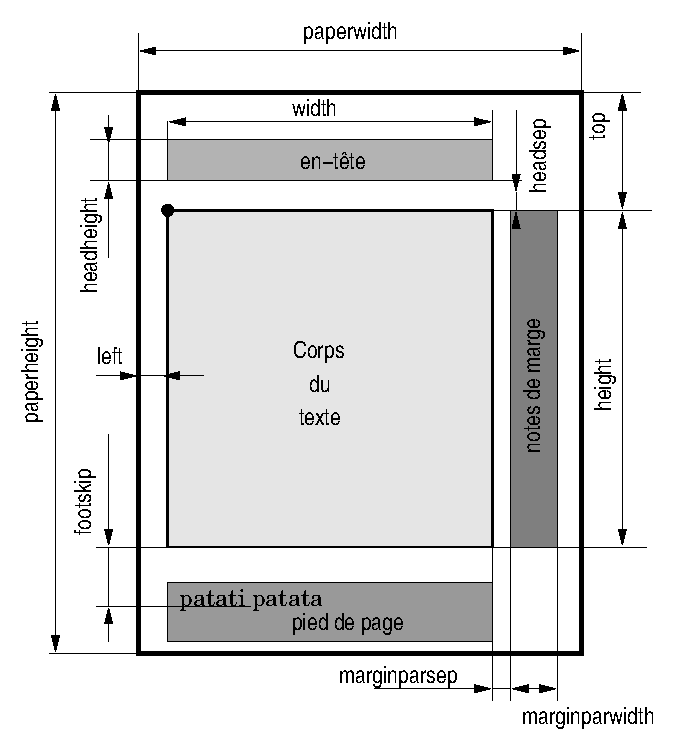
\includegraphics{img/geometry}
    \caption{定义文档几何样式的部分尺寸}
    \label{fig:10.1}
\end{figure}

以通常的方式来讲,正如图\ref{fig:10.1}展现的,包\textsf{geometry}可以定义一定数量的尺寸。我们可以以选项的方式将这些尺寸传递给\verb|\usepackage|,也可以借助指令\verb|\geometry|。

\begin{description}
    \item[页面尺寸]%TODO 此处如何换行,下同
    
\begin{itemize}
    \item 若使用预定义中的格式,可以使用\dm{a4paper}、\dm{a5paper}等。
    \item 若要自由地指定纸张尺寸,例如针对会使用碎纸机销毁的文档的尺寸,可以使用\dm{paperwidth=}\codereplace{尺寸}和\dm{paperheight=}\codereplace{尺寸}。
\end{itemize}

\item[文本]

\begin{itemize}
    \item 可以使用\dm{body=\{\codereplace{宽度},\codereplace{高度}\}};
    \item 也可以使用\dm{width=}\codereplace{宽度}和\dm{height=}\codereplace{高度};
    \item 文本在页面内的位置由参考点确定,可以使用\dm{top=}\codereplace{纵向位置}和\dm{left=}\codereplace{水平位置}确定参考点位置。
\end{itemize}

\item[页面顶端和底部]

\begin{itemize}
    \item 页面中为页面预留的高度可以借助神奇的表达式\dm{headheight=}\codereplace{高度}定义,页眉相对于版心的位置可以借助指令\dm{headsep=}\codereplace{空间}指定;
    \item 页脚的位置可以通过长度\dm{footskipp=}\codereplace{空间}指定,该长度可以定义版心底部和页脚第一行间的空间。
\end{itemize}

\item[页边注释] 秉承着同样的精神,页面中为边注预留的空间的宽度和位置可以借助两个长度定义:\dm{marginparwidth=}\codereplace{宽度}和\dm{marginparsep=}\codereplace{空间}
\end{description}

\begin{exclamation}
包geometry中,涉及页眉、页脚、边注的尺寸默认算作版心\emph{外}的部分。有一些指令可以将这些尺寸中的一个或多个包含到版心内部来完成计算。例如,我们可以说“我希望版心宽度为10厘米,包含边注”。关于更多相关细节,请参阅包文档。
\end{exclamation}

\section{页眉和页脚}

版心上下的空间分别成为页眉和页脚,可以借助包\textsf{fancyhdr}来定制。定制的基本原则很简单\jz{
    在读完接下来的内容后,你无疑会开始质疑这里说的“简单”一词……
},只需要使用以下指令来指明我们想要使用借助包\textsf{fancyhdr}定义的页眉和页脚。该包默认会在页面下方和页脚上方生成一条水平线段,线段粗细分别由\verb|\footrulewidth|和\verb|\headrulewidth|定义。接下来,我们使用以下指令:

\begin{itemize}
    \item \verb|\fancyhead|,来定义页眉;
    \item \verb|\fancyfoot|,来定义页脚。
\end{itemize}

这两条指令都可以接收由一个或两个以下字符组成的序列构成的参数:

\begin{itemize}
    \item \dm{E}或\dm{O},用于指明页码的奇偶性(偶数即\emph{even},奇数即\emph{odd});
    \item \dm{R}、\dm{L}或\dm{C},用于指明我们想在哪个位置生成信息,分别指代右侧、左侧或居中。
\end{itemize}

示例如下:

\begin{dmd}
\begin{verbatim}
\fancyhf{} % 清除页面并开始
% 【页眉】
% 作者姓名首字母偶数页靠右,奇数页靠左:
\fancyhead[RE,LO]{VL}
% 页码居中:
\fancyhead[C]{\thepage}
% 节号奇数页靠右,
% 偶数页靠左:
\fancyhead[LE,RO]{\thesection}
% 【页脚】
% 图片奇数页靠右,偶数页靠左:
\fancyfoot[RO,LE]{
\includegraphics[height=4ex]{punch}}
% 标题奇数页靠右,偶数页靠左:
\fancyfoot[LO,RE]{%
    关于\LaTeX{}的那些你想知道的问题}
% 线条粗细
\renewcommand{\footrulewidth}{3pt}
\end{verbatim}
\end{dmd}

\fancyhf{} 
\fancyhead[RE,LO]{VL}
\fancyhead[C]{\thepage}
\fancyhead[LE,RO]{\thesection}
\fancyfoot[RO,LE]{
\includegraphics[height=4ex]{punch}}
\fancyfoot[LO,RE]{关于\LaTeX{}的那些你想知道的问题}
\renewcommand{\footrulewidth}{3pt}

\subsection{章首页的情况}

在类型\dm{book}中,\LaTeX 会自动为每章的第一页调用风格\dm{plain}。为了使包\textsf{fancyhdr}为这些页面定义新风格,可以使用如下指令:

\begin{dmd}
\begin{verbatim}
% 章首页的情况 
\fancypagestyle{plain}{%
    \fancyhf{}% 全部清空 
    \fancyfoot[C]{\thepage}% 页面底部的页码
    % 清空所有线条
    \renewcommand{\headrulewidth}{0pt}% 
    \renewcommand{\footrulewidth}{0pt}}
\end{verbatim}
\end{dmd}

可以注意到,本书各章的章首正是采用了这种风格……

\subsection{章首前的空白页}

在类型\dm{book}的双面模式下(正是本文档对应的情况),\LaTeX 会默认在奇数页——这在排版术语中称作“单面”(belle page)——开始新的一章。为了实现这一点,\LaTeX 在不同的内部指令中调用了指令\verb+\cleardoublepage+。这样可以在必要时在章的首页前插入一个空白页。默认情况下,该空白页会带有目前使用的页眉和页脚。在本文档中,我们针对这些页面修改了文件\dm{latex.ltx}中的指令\verb|\cleardoublepage|,指定了一种“空白”的风格:%TODO 还没搞

\begin{dmd}
\begin{verbatim}
\renewcommand{\cleardoublepage}{% 重定义该指令
    \clearpage\ifodd\c@page\else
    \hbox{}
    \vspace*{\fill}
    \thispagestyle{empty}% 添加此行 
    \newpage
    \fi}
\end{verbatim}
\end{dmd}

你可以翻阅本书,看看章首前的页面是否是空白的……

\subsection{标记的机制}

你无疑已经注意到了,本书的页眉带有一些与文本相关的内容。实际上,针对偶数页(出现在左侧的页面),我们插入了章标题;针对奇数页(出现在右侧的页面),我们插入了该页出现的最后一节的节标题。\LaTeX 部署了一种\emph{标记}机制,使得我们可以实现这一点。这里将尝试解释这种机制。

\begin{exclamation}
这里不妨解释一下:\LaTeX 和\TeX 生成一个页面是,它们会根据从所涉页面收集来的信息来制备页眉和页脚。因此,生成页眉和页脚是编译页面的后置步骤。
\end{exclamation}

\subsubsection{指令\dm{\backslash markboth}和\dm{\backslash markright}}

设有以下指令:

\begin{dmd}
\backslash markboth\{\codereplace{文本$_{\mbox{左}}$}\}\{\codereplace{文本$_{\mbox{右}}$}\}
\end{dmd}

或:

\begin{dmd}
\backslash markright\{\codereplace{文本}\}
\end{dmd}

想象参数\codereplace{文本$_{x}$}存储在栈和队列中。根据这种想法,有:

\begin{itemize}
    \item \verb|\markboth|将\codereplace{文本$_{\mbox{左}}$}入栈,将\codereplace{文本$_{\mbox{右}}$}存入队列;
    \item \verb|\markright|将\codereplace{文本}存入队列。
\end{itemize}

在一个页面中,这两个“标记”指令可以调用多次,也可以一次都不调用。在\TeX 结束版心的排版,在生成页眉和页脚时,会探索栈和队列的参数。这借助了以下指令:

\begin{itemize}
    \item \verb|\leftmark|返回栈顶,即\emph{上一次调用}\verb|\markboth|时的\codereplace{文本$_{\mbox{左}}$};
    \item \verb|\rightmark|返回队列头,即\emph{第一次调用}\verb|\markboth|时的\codereplace{文本$_{\mbox{右}}$},或\emph{第一次调用}\verb|\markbot|时的\codereplace{文本}。
\end{itemize}

\begin{ii}
供你参考的是,作者使用了这些指令来生成了带有几十个名称和照片的相册。这里的思路是去探索通过页眉显示页面上第一个和最后一个名称的机制——这种页眉跟字典很像。为了实现这个目的,只需要为每个人(包含名称和照片)调用以下指令:

\begin{dmd}
\backslash markboth\{\codereplace{老铁的名称}\}\{\codereplace{老铁的名称}\}
\end{dmd}

接下来,在左侧页眉中插入指令\verb|\rightmark|

\end{ii}